\chapter{Networking Technologies}
\label{ch:networkingtechnologies}

\section{Networking in GRAMOC}

Because GRAMOC is a client-server architecture, a common way of communication had to be developed. This development process resulted in GSDEP.

\section{GSDEP}

GRAMOC Sensor Data Exchange Protocol (GSDEP) is GRAMOC's Network Protocol that is used for sending large amounts of sensor data to the clients. It is built on top of the TCP/IP stack \cite{rfc793, rfc791}.

\subsection{Data Flow}
\label{sec:networking_data-flow}

Figure \ref{fig:handshake} depicts the handshake performed by GSDEP that is based on TCP's three-way handshake. The Client sends a synchronize (SYN) message to the server to let it know that it wants to connect. If the server can accept new Clients it returns an acknowledgment message (ACK). The client then also returns this acknowledgment message to inform the server that it is indeed connected. The connection now is established.

\begin{figure}[H]
	\centering
	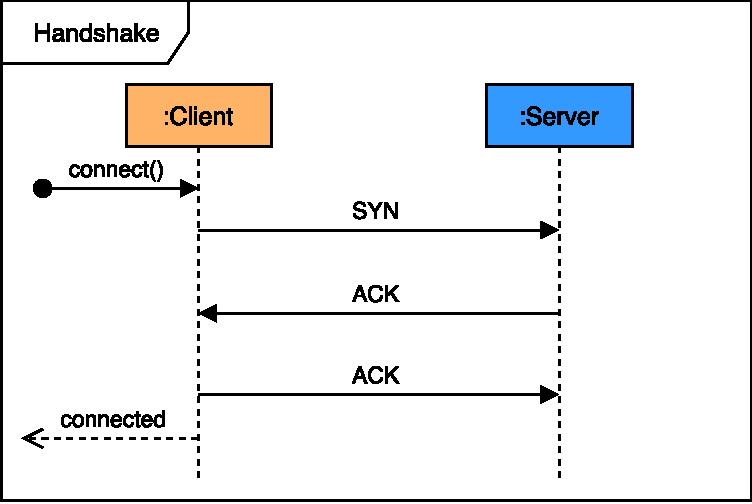
\includegraphics[width=8cm,keepaspectratio]{gsdep_handshake}
	\caption{TCP-like three way handshake performed on client connect}
	\label{fig:handshake}
\end{figure}

If a client wants to disconnect from the server it will send a disconnect message (FIN) to the server. Before it actually disconnects, it has to wait for the server to finish cleaning up and return the FIN packet. After the client has received this message, it can close the connection and shut down. This procedure is shown in Figure \ref{fig:disconnect}.

\begin{figure}[H]
	\centering
	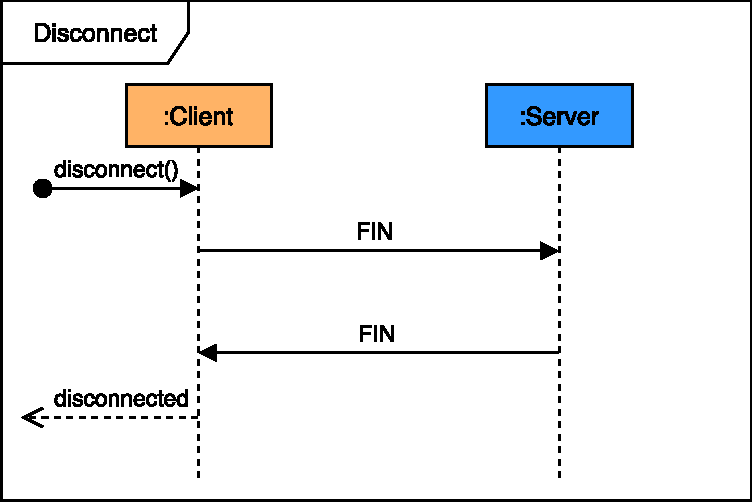
\includegraphics[width=8cm,keepaspectratio]{gsdep_disconnect}
	\caption{Two way handshake performed on client disconnect}
	\label{fig:disconnect}
\end{figure}

\subsection{Data Interchange Format}

Every message consists of a header and the actual payload that is transmitted. The header includes additional information that is used by the other end to only read one message (see \ref{sec:messageframing}), to differentiate between different kinds of messages (see \ref{sec:channels}) and to rebuild the message data to its correct data type. As depicted in Figure \ref{fig:packet}, the header consists of 4 bytes message length and 2 bytes each for data type and channel.

\begin{figure}[H]
	\centering
	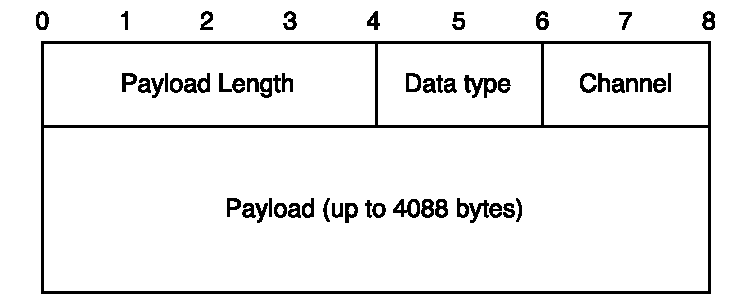
\includegraphics[width=8cm,keepaspectratio]{gsdep_packet}
	\caption{Structure of one packet sent by GSDEP}
	\label{fig:packet}
\end{figure}

\subsection{Commands}
\label{sec:networking_command}

Commands are special messages that are sent to the endpoint that require further action to be taken. These commands can either be used during the connect or disconnect handshakes, or to request data.

\begin{table}[H]
	\centering
	\begin{tabular}{| l | l | p{5cm} |}
	\hline
	\textbf{Command} & \textbf{Used by} & \textbf{Meaning} \\ \hline
	SYN & client & Tells the server that a new client wants to connect \\ \hline
	ACK & server \& client & Tells the other end that it acknowledges the previous command \\ \hline
	FIN & server \& client & Tells the other end that it will disconnect \\ \hline
	STD & client & Tells the server that the client requests data\\ \hline
	SPD & client & Tells the server that the client rejects data\\
	\hline
	\end{tabular}
	\caption{Commands sent by one of the connection partners and what they do}
	\label{tab:commands}
\end{table}

\subsection{Channels}
\label{sec:channels}

In the case of GRAMOC, where large amounts of data are received in short periods of time, it is crucial to differentiate between communication data and sensor data in split seconds. To accomplish this a 2 byte unsigned short is included in the packet header. This information can the be used to tell apart these two types of data.

\begin{table}[H]
	\centering
	\begin{tabular}{| l | c |}
	\hline
	\textbf{Channel} & \textbf{Value} \\ \hline
	Communication & 1 \\ \hline
	Data & 2 \\
	\hline
	\end{tabular}
	\caption{Channels used to distinguish between message types}
	\label{tab:channels}
\end{table}

\subsection{Message framing}
\label{sec:messageframing}
Because TCP operates with streams of data and not packets of data, messages have to be framed so that the receiving end knows what one message is. This can be done in two ways. \cite{MessageFramingCleary,MessageFramingSkotzko}

\subsubsection{Length Prefixing}

One method of Message framing is to prefix each message with its length. When doing so the format of the message length has to be stated explicitly. In the case of GSDEP that is a ``4 byte unsigned integer''.

\paragraph{Sending}

First, the message has to be encoded into its binary representation. To send this message, the length followed by the binary encoded message simply has to be sent.

\paragraph{Receiving}

Receiving one message is done by first reading into a buffer of specified length (in this case the buffer would be 4 bytes long). Then the message is read into a second buffer with the just read length. When this buffer is full, one message has been read.

\subsubsection{Delimiters}

\paragraph{Sending}

Messages can also be framed by using delimiters. This can be done by sending a special character between each message. This character can either be a character that does not show up in actual messages (e.g. a Null character), or a character that is present in a message. If the second approach is used, every message has to be run through an escaping process which replaces these characters in the messages.

\paragraph{Receiving}

Receiving delimited messages is relatively straightforward. One message is read when a delimiter is reached. This message has to be passed to an unescaping function when a delimiter character is chosen that can exist in messages.

\subsubsection{Security Concerns}

Whichever solution is chosen, each solution has to provide code regarding Denial of Service (DoS) attacks. Wether a very big message length or large amounts of data without a delimiter are received, both can result in Out of Memory Exceptions.
